% This example file for NIH submissions was originally written
% by Bruce Donald (http://www.cs.duke.edu/brd/).
%
% You may freely use, modify and/or distribute this file.
%
\documentclass[11pt]{nih}
%\documentclass[11pt,draft]{nih}
%\documentclass{article}
%\documentclass[12pt]{article}%
% last revision:
\def\mydate{2005-06-09 13:58:03 brd}


%%%%%%% Two column control
\newif\ifdotwocol
\dotwocoltrue   % two col
%\dotwocolfalse   % one col
\long\def\twocol#1#2{\ifdotwocol{#1}\else{#2}\fi}
%%%%%%%

\def\mybeforeequation{\footnotesize}
%\def\mybeforeequation{\small}
%\def\mybeforeequation{}

\def\myafterequation{\renewcommand\baselinestretch{1.1}}
%\def\myafterequation{}

%%%%%%%%%%%%%%%%
%%%%%%%%%%%%%%%%

\def\citeusmark{$^{\textstyle \star}$}
\def\citeus#1#2{\cite{#1}}

\def\crow#1#2{#2}

%\usepackage{denselists}
%\usepackage{scaledfullpage}
\usepackage[dvips]{graphicx}
\usepackage{color}
\usepackage{boxedminipage}
\usepackage{amsfonts}
\usepackage{mathtools}
\usepackage{mathrsfs}
\usepackage{amsmath}
\usepackage{amssymb}
\usepackage{url}
\usepackage{wrapfig}
\usepackage[font=small,format=plain,labelfont=bf,up,textfont=it,up]{caption}
%\usepackage{subfig}
\usepackage{multirow}
%\usepackage{times}
%\usepackage{nih}		% PHS 398 Forms
%\usepackage{nihblank}		% For printing on Blank PHS 398 Forms
%\usepackage{confidential}
\usepackage[subrefformat=parens,labelformat=parens]{subfig}  %% subfigure referencing
\usepackage{newclude}

\usepackage{colortbl}
\usepackage[table]{xcolor}

\usepackage{soul}
\usepackage{verbatim}

\def\Paper{grant application}
\def\paper{application}
\def\refappendix{Sec.}


\def\poster{(Poster)}

%Note from brd
\long\def\todo#1{{\bf{To do:}} #1}
%\long\def\todo#1{}V-neck
\def\ICRA{IEEE International Conference on Robotics and Automation (ICRA)}

\long\def\squeezable#1{#1}

%\def\a5{$\alpha_{_5}$

\def\a5{5}

\def\mycaptionsize{\normalsize}
\def\mycaptionsize{\small}
\def\mycaptionsize{\small}


%\def\mycaptionsize{\footnotesize}
%\def\mycodesize{\footnotesize}
%\def\myeqnsize{\small}

\def\sheading#1{{\bf #1:}\ }
\def\sheading#1{\subsubsection{#1}}

\usepackage[compact]{titlesec}
%\titlespacing{\section}{0pt}{2ex}{1ex}
%\titlespacing{\subsection}{0.5pt}{1ex}{0.5ex}
%\titlespacing{\subsubsection}{0pt}{0.5ex}{0ex}

%\def\sheading#1{\bigskip {\bf #1.}}

\def\ssheading#1{\noindent {\bf #1.}\ }

\newtheorem{hypothesis}{Hypothesis}
\long\def\hyp#1{\begin{hypothesis} #1 \end{hypothesis}}

\def\cbk#1{[{\em #1}]}

\def\R{\mathbb{R}}
\def\midv{\mathop{\,|\,}}
\def\Fscr{\mathcal{F}}
\def\Gscr{\mathcal{G}}
\def\Sscr{\mathcal{S}}
\def\set#1{{\{#1\}}}
\def\edge{\!\rightarrow\!}
\def\dedge{\!\leftrightarrow\!}
\newcommand{\EOP}{\nolinebreak[1]~~~\hspace*{\fill} $\Box$\vspace*{\parskip}\vspace*{1ex}}
%my way of doing starred references
\newcommand{\mybibitem}[1]{\bibitem{#1}
\label{mybiblabel:#1}}
\newcommand{\BC}{[}
\newcommand{\EC}{]}
\newcommand{\mycite}[1]{\ref{mybiblabel:#1}\nocite{#1}}
\newcommand{\starcite}[1]{\ref{mybiblabel:#1}\citeusmark\nocite{#1}}


\def\degree{$^\circ$}
\def\R{\mathbb{R}}
\def\Fscr{\mathcal{F}}
\def\set#1{{\{#1\}}}
\def\edge{\!\rightarrow\!}
\def\dedge{\!\leftrightarrow\!}

\long\def\gobble#1{}
\def\Jigsaw{{\sc Jigsaw}}
\def\ahelix{\ensuremath{\alpha}-helix}
\def\ahelices{\ensuremath{\alpha}-helices}
\def\ahelical{$\alpha$-helical}
\def\bstrand{\ensuremath{\beta}-strand}
\def\bstrands{\ensuremath{\beta}-strands}
\def\bsheet{\ensuremath{\beta}-sheet}
\def\bsheets{\ensuremath{\beta}-sheets}
\def\hone{{\ensuremath{^1}\rm{H}}}
\def\htwo{{$^{2}$H}}
\def\cthir{{\ensuremath{^{13}}\rm{C}}}
\def\nfif{{\ensuremath{^{15}}\rm{N}}}
\def\hn{{\rm{H}\ensuremath{^\mathrm{N}}}}
\def\hnone{{\textup{H}\ensuremath{^1_\mathrm{N}}}}
\def\ca{{\rm{C}\ensuremath{^\alpha}}}
\def\catwel{{\ensuremath{^{12}}\rm{C}\ensuremath{^\alpha}}}
\def\ha{{\rm{H}\ensuremath{^\alpha}}}
\def\cb{{\rm{C}\ensuremath{^\beta}}}
\def\hb{{\rm{H}\ensuremath{^\beta}}}
\def\hg{{\rm{H}\ensuremath{^\gamma}}}
\def\dnn{{\ensuremath{d_{\mathrm{NN}}}}}
\def\dan{{\ensuremath{d_{\alpha \mathrm{N}}}}}
\def\jconst{{\ensuremath{^{3}\mathrm{J}_{\mathrm{H}^{\mathrm{N}}\mathrm{H}^{\alpha}}}} }
\def\cbfb{{CBF-$\beta$}}

\newtheorem{defn}{Definition}
\newtheorem{claim}{Claim}

    \gobble{
    \psfrag{CO}[][]{\colorbox{white}{C}}
    \psfrag{OO}[][]{\colorbox{white}{O}}
    \psfrag{CA}[][]{\colorbox{white}{\ca}}
    \psfrag{HA}[][]{\colorbox{white}{\ha}}
    \psfrag{CB}[][]{\colorbox{white}{\cb}}
    \psfrag{HB}[][]{\colorbox{white}{\hb}}
    \psfrag{HN}[][]{\colorbox{white}{\hn}}
    \psfrag{N15}[][]{\colorbox{white}{\nfif}}
    \psfrag{dnn}[][]{\dnn}
    \psfrag{dan}[][]{\dan}
    \psfrag{phi}[][]{$\phi$}
    }

\newenvironment{closeenumerate}{\begin{list}{\arabic{enumi}.}{\topsep=0in\itemsep=0in\parsep=0in\usecounter{enumi}}}{\end{list}}
\def\CR{\hspace{0pt}}           % ``invisible'' space for line break

\newenvironment{closeitemize}{\begin{list}{\textbullet }{\topsep=0.05in\itemsep=0.02in\parsep=0.0in\usecounter{enumi}}}{\end{list}}


\newif\ifdbspacing
%\dbspacingtrue  % For double spacing
\dbspacingfalse  % For normal spacing

\ifdbspacing
  \usepackage{setspace}
 \doublespacing
 \newcommand{\capspacing}{\doublespace\mycaptionsize}
\else
 \newcommand{\capspacing}{\mycaptionsize}
\fi

\def\rulefigure{\smallskip\hrule}

% \def\codesize{\normalsize}
\def\codesize{\small}

% Can use macros \be, \ee, \en as shortcuts
%  for \begin{enumerate}, \end{enumerate}, \item
%  respectively.

\def\be{\begin{enumerate}}   % Begin Enumerate
\def\ee{\end{enumerate}}     % End Enumerate
\def\en{\item}               % ENtry (item)
\def\bi{\begin{itemize}}     % Begin Itemize
\def\ei{\end{itemize}}       % End Itemize
\def\bv{\begin{verbatim}}    % Begin Verbatim
\def\ev{\end{verbatim}}      % End Verbatim

\def\matlab{{\sc matlab} }
\def\amber{{\sc amber} }
\def\KS{{$K^*$}}
\def\KSM{{K^*}} % K-Star Math
\def\KSTM{{\tilde{K}^*}}  % K-Star Tilde Math (appx K*)
\def\KOP{{$K^{\dagger}_{o}$}}  % K-Star Optimal partial
\def\KOPM{{K^{\dagger}_{o}}}  % K-Star Optimal partial Math
\def\KP{{$K^{\dagger}$}}  % K-Star partial
\def\KPM{{K^{\dagger}}}  % K-Star partial Math
\def\KTPM{{\tilde{K}^{\dagger}}}  % K-Star Tilde partial Math
\def\KD{{$K_{_D}$}}
\def\KA{{$K_{_A}$}}
\def\qpM{{q_{_P}}}
\def\qlM{{q_{_L}}}
\def\qplM{{q_{_{PL}}}}
\def\qSplM{{q^*_{_{PL}}}}
\def\KSO{{$K^*_{o}$}} % K-Star Optimal
\def\KSOM{{K^*_{o}}}  % K-Star Optimal Math
\def\CBFB{{CBF-$\beta$}}   % Core binding factor beta
\def\argmin{\mathop{\mathrm{argmin}}}
\def\rhl#1{{\em \underline{RYAN}: *\{{#1}\}*}}
\def\set#1{{\left\{ #1 \right\}}}
\def\Escr{{\mathcal{E}}}
\def\Jscr{{\mathcal{J}}}
\def\Kscr{{\mathcal{K}}}
\def\th{{$^{{\mathrm{th}}}$}}

\newtheorem{proposition}{Proposition}
\newtheorem{lemma}{Lemma}



%for the title page
\newcommand{\HRule}{\rule{\linewidth}{0.5mm}}


\usepackage{colortbl}

\graphicspath{{figs/}}

\begin{document}

\begin{titlepage}

\begin{center}

% Upper part of the page
%\includegraphics[width=10cm]{DomeWordSingleMED.png}\\[1cm]

\textsc{\Large Comprehensive Exam and Project Proposal}\\[0.5cm]

% Title
\HRule \\[0.4cm]
{\LARGE \bfseries
    Super-resolution of diffusion-weighted images using enhanced multi-spectral classification results
}\\[0.4cm]

\HRule \\[1.5cm]

\end{center}

\begin{flushleft}
\LARGE{Ali Ghayoor} \\
\large{ali-ghayoor@uiowa.edu} \\

\vspace{60pt} %120
\large{Wednesday, March $23^{rd}$, 2016} \\
\large{Time: 12:30 - 2:30 pm} \\
\large{Room: 3210 SC}
\vspace{60pt} % 80

\Large{\textbf{Committee Members} }\\
\large{
\vspace{10pt}
{\bf Johnson, Hans J., Ph.D. (Chair) }\\
Department of Electrical \& Computer Engineering \\
\vspace{10pt}
{\bf Christensen, Gary E., Ph.D.}\\
Department of Electrical \& Computer Engineering \\
\vspace{10pt}
{\bf Jacob, Mathews, Ph.D.}\\
Department of Electrical \& Computer Engineering \\
\vspace{10pt}
{\bf Garvin, Mona K., Ph.D.}\\
Department of Electrical \& Computer Engineering \\
\vspace{10pt}
{\bf Magnotta, Vincent A., Ph.D.}\\
Department of Biomedical Engineering \\
\vspace{10pt}
{\bf Vaidya, Jatin G., Ph.D.}\\
Department of Psychiatry \\
}
\end{flushleft}

\end{titlepage}

\bigskip

\appendix

%\mydate

%\begin{comment}
%-----------------------------------------------
\setcounter{secnumdepth}{5}

\titleformat{\paragraph}
{\normalfont\normalsize\bfseries}{\theparagraph}{1em}{}
\titlespacing*{\paragraph}
{0pt}{3.25ex plus 1ex minus .2ex}{1.5ex plus .2ex}
%-----------------------------------------------
%\end{comment}

\tableofcontents
\newpage

\setcounter{page}{1} % or whatever

\include*{Introduction}
\include*{ClinicalBackground}
\include*{ResearchDesignAndPreliminaryResults}
%\section{Research Design and Methods}
Following explains the plans to accomplish the specific aims outlined in section \ref{specificAims}.


%use the complementary information provided by DWI processing pipeline explained in preliminary work related to Aim 1 (section \ref{subsection:dwi_processing_pipline}) to enhance the classification and registration results previously generated from structural MRI data alone.

\subsection{Enhance tissue classification by a fuzzy k-Nearest Neighbor classifier using complementary information derived from diffusion-weighted imaging data}
\label{researchPlan:classification}
Preliminary results of section \ref{subsection:fuzzy_knn_method} proved enhancements in tissue classification quality by extension of $EM$-based classification method using a fuzzy $kNN$ classifier.
This new infrastructure achieved better classification results even if we only used original structural MR imaging inputs. This motivates us to expect even more improvements in the results by incorporating new modality information, derived from diffusion imaging data, into the training of fuzzy k-NN algorithm. The output rotationally invariant scalars (RISs) from DWI processing pipeline, explained in section \ref{subsection:dwi_processing_pipline}, provide valuable complementary information to the structural scans so that tissue classification results are improved.
\newline

\noindent Nevertheless, the proposed classification framework in section \ref{subsection:fuzzy_knn_method},
cannot handle multi-spectral data when the input modality scans are not in approximately the same spatial resolution. The current implementation of $kNN$ classifier assumes that the outputs of the previous $EM$ classification step all have been resampled to a consistent isotropic $1\times1\times1$ $mm^3$ voxel lattice. However, the DWI scans and their derived rotationally invariant scalars (RISs) are in a different voxel space with a lower spatial resolution ($2\times2\times2$ $mm^3$) than their corresponding structural MR T1/T2 weighted scans. This misalignment between voxel-sizes and voxel-locations causes partial volume effect (PVE) at tissue boundaries
%that means many voxels contain more than one tissue type.
that means voxels at the boundaries contain a mixture of tissue types. Using these voxels in training of the fuzzy k-NN algorithm will adversely affect the performance of the classifier and results in less accurate tissue classification.
\newline

\noindent Figure \ref{fig:pve} shows the PVE issue in a simplified $1D$ demonstration, where $1D$ MRI signals from three different image modalities (T1, T2 and DWI) are demonstrated near a boundary of two types of matter in brain (Gray matter and White matter).
The MRI works by detecting the magnetic particles in atoms within cells and sending electromagnetic pulses at different rates and strength through the body. The different types of biological matter give off distinguishing levels of energy when they are placed in a magnetic field. These energy signals, collected by the electromagnetic receivers, are quantized and sampled into discrete voxel segments in an output image scan. The differing signal levels of tissue types display as separate intensities in the output image. In an MRI scanning session, a number of different scans are run. Depending on how they measure the relaxation of the magnetic particles, a variety of modality images with different contrasts are acquired. For example, in a T1 scan, gray matter gives off a low signal and looks darker than the white matter that gives off a higher signal and looks pale gray, but this is inverse in T2 and DWI scans.
\newline

\noindent Although objects of interest usually form coherent contiguous shapes with clear anatomical borders, the representation of tissue boundaries in discretized image scans is not perfectly in agreement with real anatomy because of error in image discretization.
First, the measurement of MRI signals is not perfect due to hardware limitations and the presence of noise in the input image, so the collected signals are quantized in several intermediate levels in boundary regions.
Then, quantized signals are mapped in discretized segments of spatial domain. A value is assigned to each voxel of the image based on the average of samples taken during the spatial location of that voxel.
If the image has a low spatial resolution with large voxel sizes, it is most likely that many voxels are placed in two different anatomical regions, so their value reflects a partial volume composition of more than one tissue type.
\newline

\noindent Partial volume composition affects a larger number of spatial samples when the multimodal information come from the modality scans with very different resolution and origin.
In figure \ref{fig:pve}, the MRI signals are sampled at the center points of the lattice segments in the T1 scan. When only two T1 and T2 modalities with comparable resolutions are used, we have more pure plugs since only two spatial samples are affected by partial volume composition (specified in a red rectangle).
However, adding new modality information from a low resolution scan introduces the partial volume effect to a larger number of spatial samples. The affected samples are represented by a question mark as they reflect more than one tissue type.
\newline

\noindent A careful consideration should be made to only use pure plugs for training of classification module.
As anatomical objects have coherent continues shapes, pure plugs have likely consistent values with their neighbors. It gives a hint to use a kernel on neighboring samples to identify pure plugs for training of classifier.

\begin{figure}[ht!]
    \begin{center}
      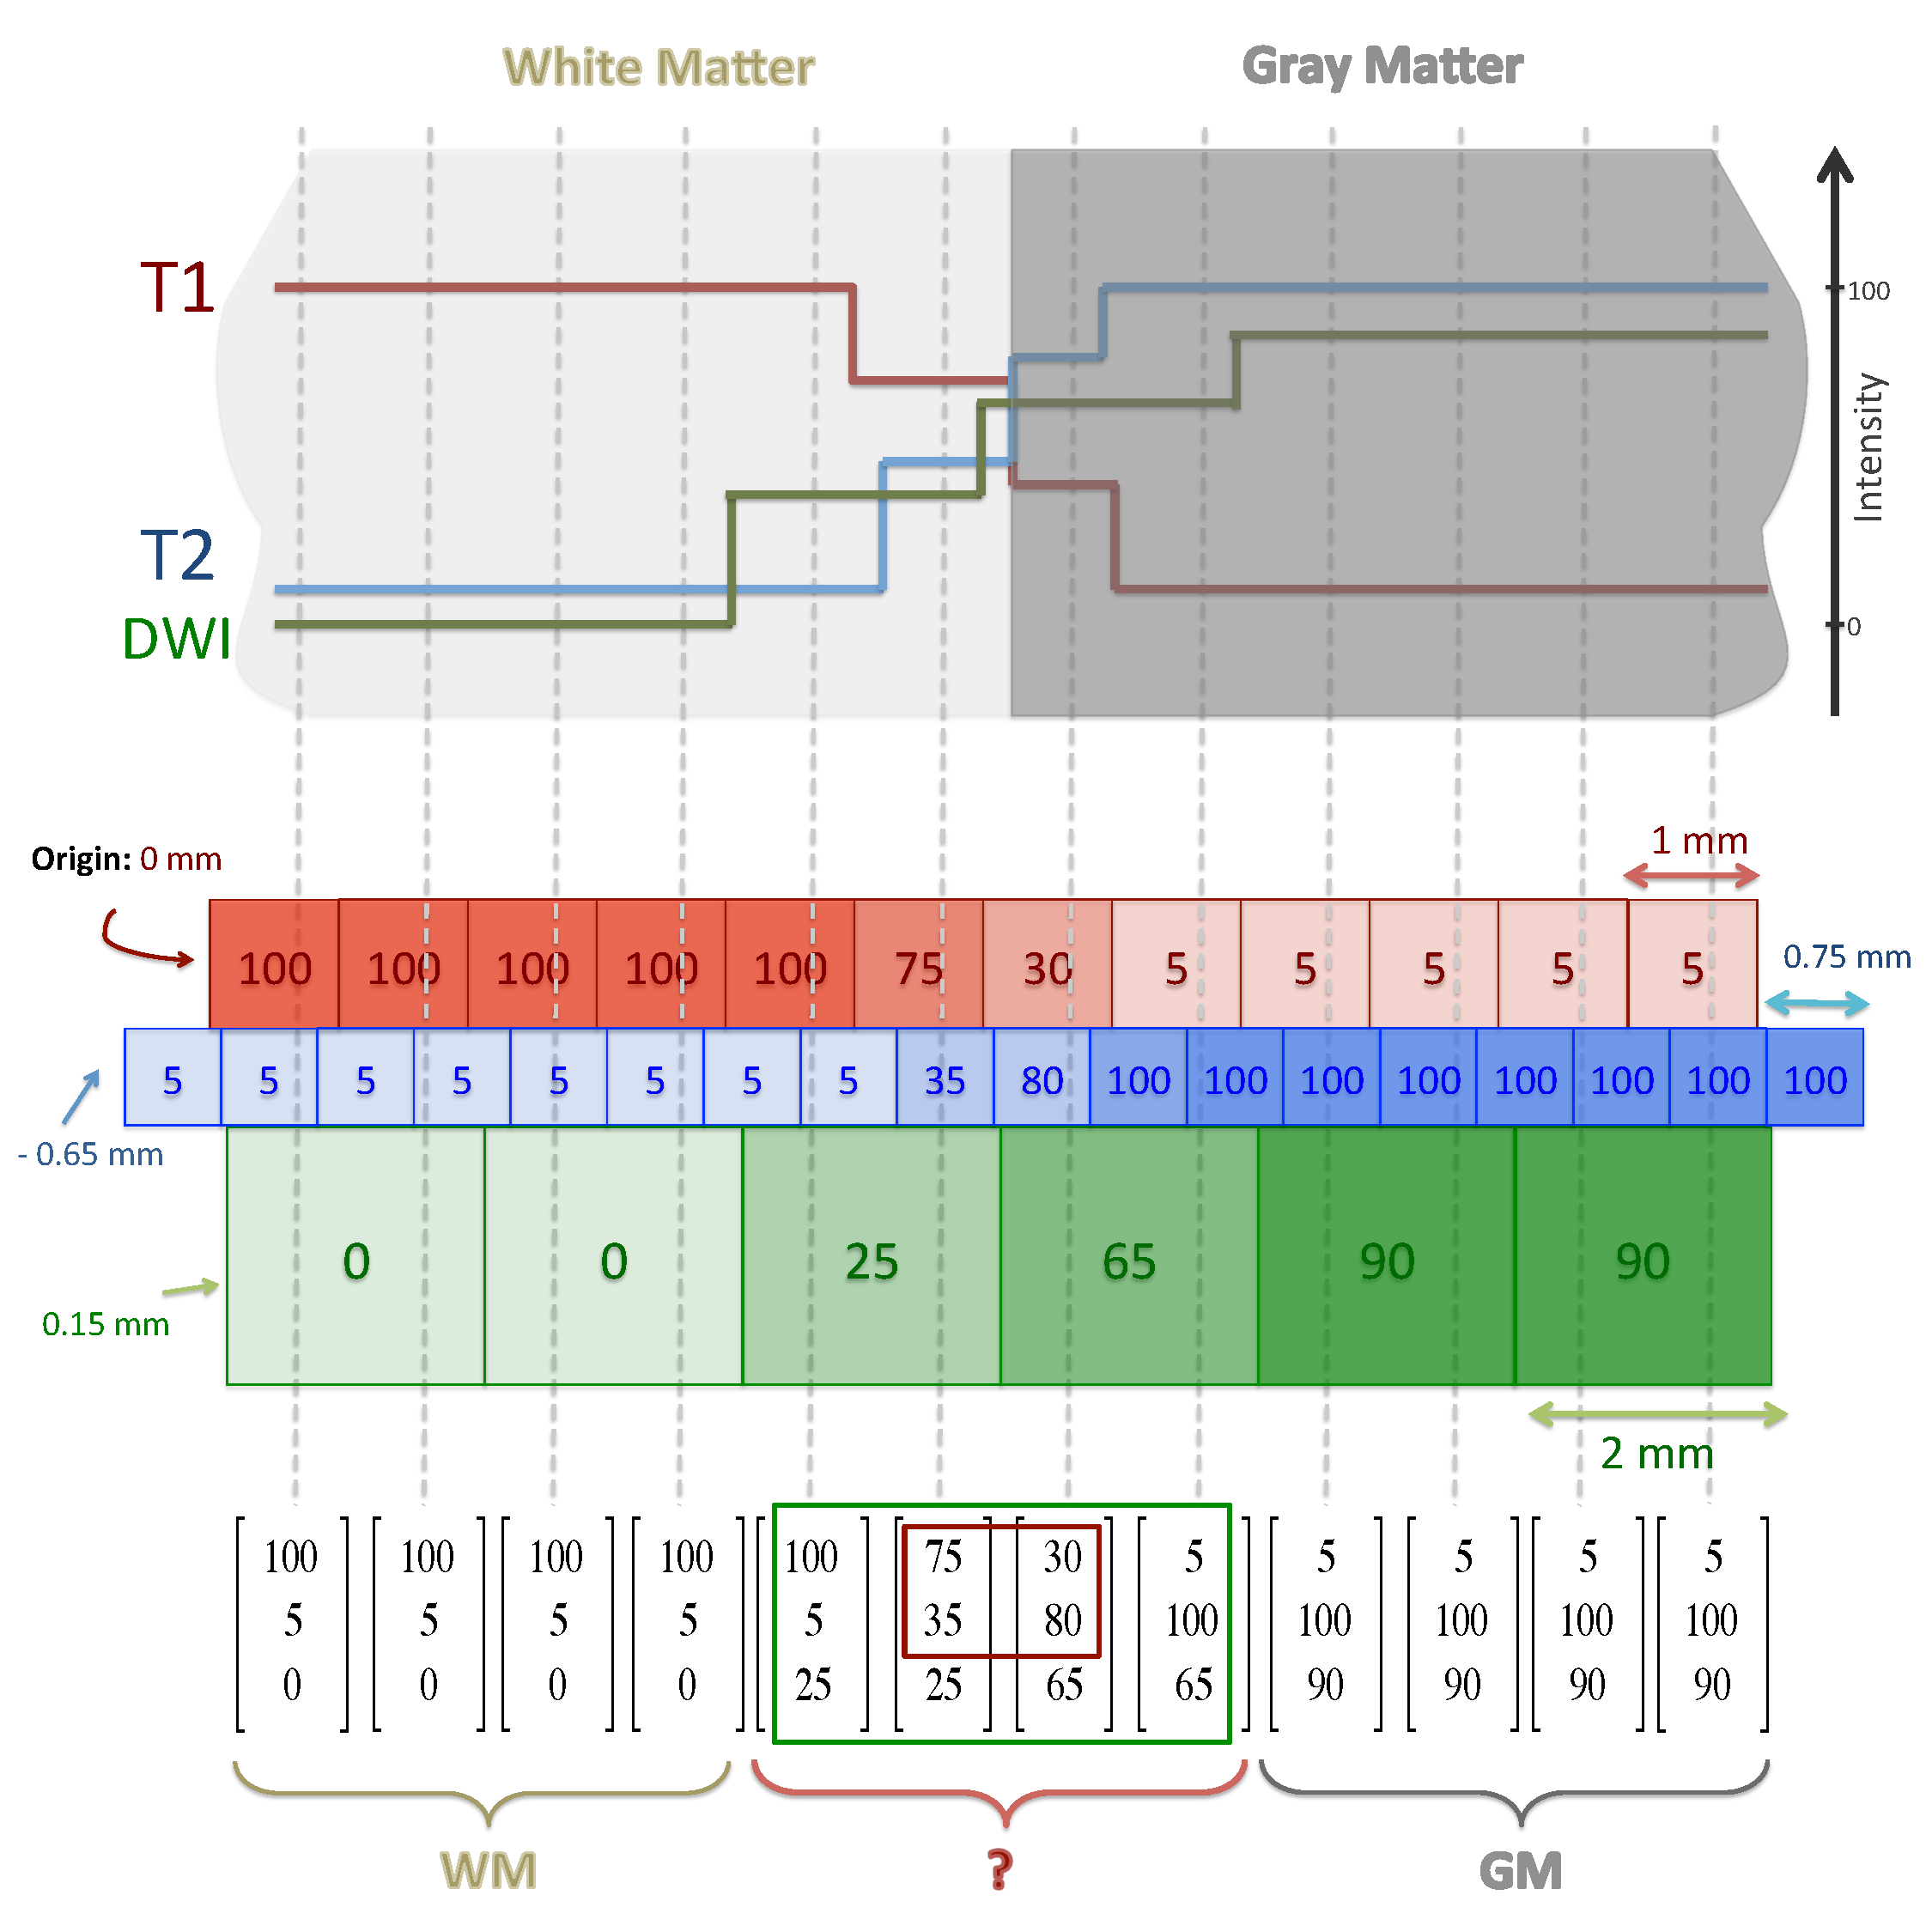
\includegraphics[width=0.85\textwidth]{./Figures/pve.pdf}
    \end{center}
    \vspace{-15pt}
    \caption{$1D$ demonstration of partial volume effect (PVE) when MRI signals of different modalities are sampled to discrete segments with differing spatial resolution and origin. The question mark represent the sample values that reflect a partial volume composition of more than one tissue type.}
    \vspace{-5pt}
    \label{fig:pve}
\end{figure}

\subsection{Super-resolution of diffusion-weighted images using the boundary curves information}
It is a common practice to acquire diffusion-weighted imaging data at a lower resolution than the structural MRI, due to the slow nature of DWI acquisition, subject motion, and the decrease in SNR with resolution. However, generation of high-resolution DWI data is highly desirable since it can simplify the interpretation of measures that correspond to anatomical regions estimated from the higher resolution morphological scans (i.e. T1/T2).
\newline

\noindent In addition to the clinical advantages, the multi-spectral data, acquired from super-resolution reconstructed diffusion-weighted images, can be incorporated into a multimodal registration framework to enhance registration quality. Previously a multi-modal registration framework was developed for ANTs \cite{Avants2008b, Avantsa} and BRAINSTools \cite{BRAINSia} that uses the information of different modality images simultaneously to compute a weighted measure of the metric. Our initial investigation on one sample dataset showed that utilizing two T1 and T2 scans in a multimodal framework produces superior results as compared to the registration method using only T1-weighted scans. It motivates us to expect even further improvement in the registration results by using new modality information acquired from super-resolution reconstructed diffusion-weighted imaging data.
\newline

\noindent Figure \ref{fig:super_resolution1} shows the mismatch between actual anatomy boundaries and the voxel borders in an image scan with low spatial resolution. Many voxels in boundary regions have an artificial value that does not belong to any specific region but reflects average composition of MRI signals acquired from more than one tissue type. Classifying these voxels into a single tissue type can cause large segmentation error. Also, it is impossible to segment a region that is smaller than the voxel area.

\begin{figure}[ht!]
    \begin{center}
      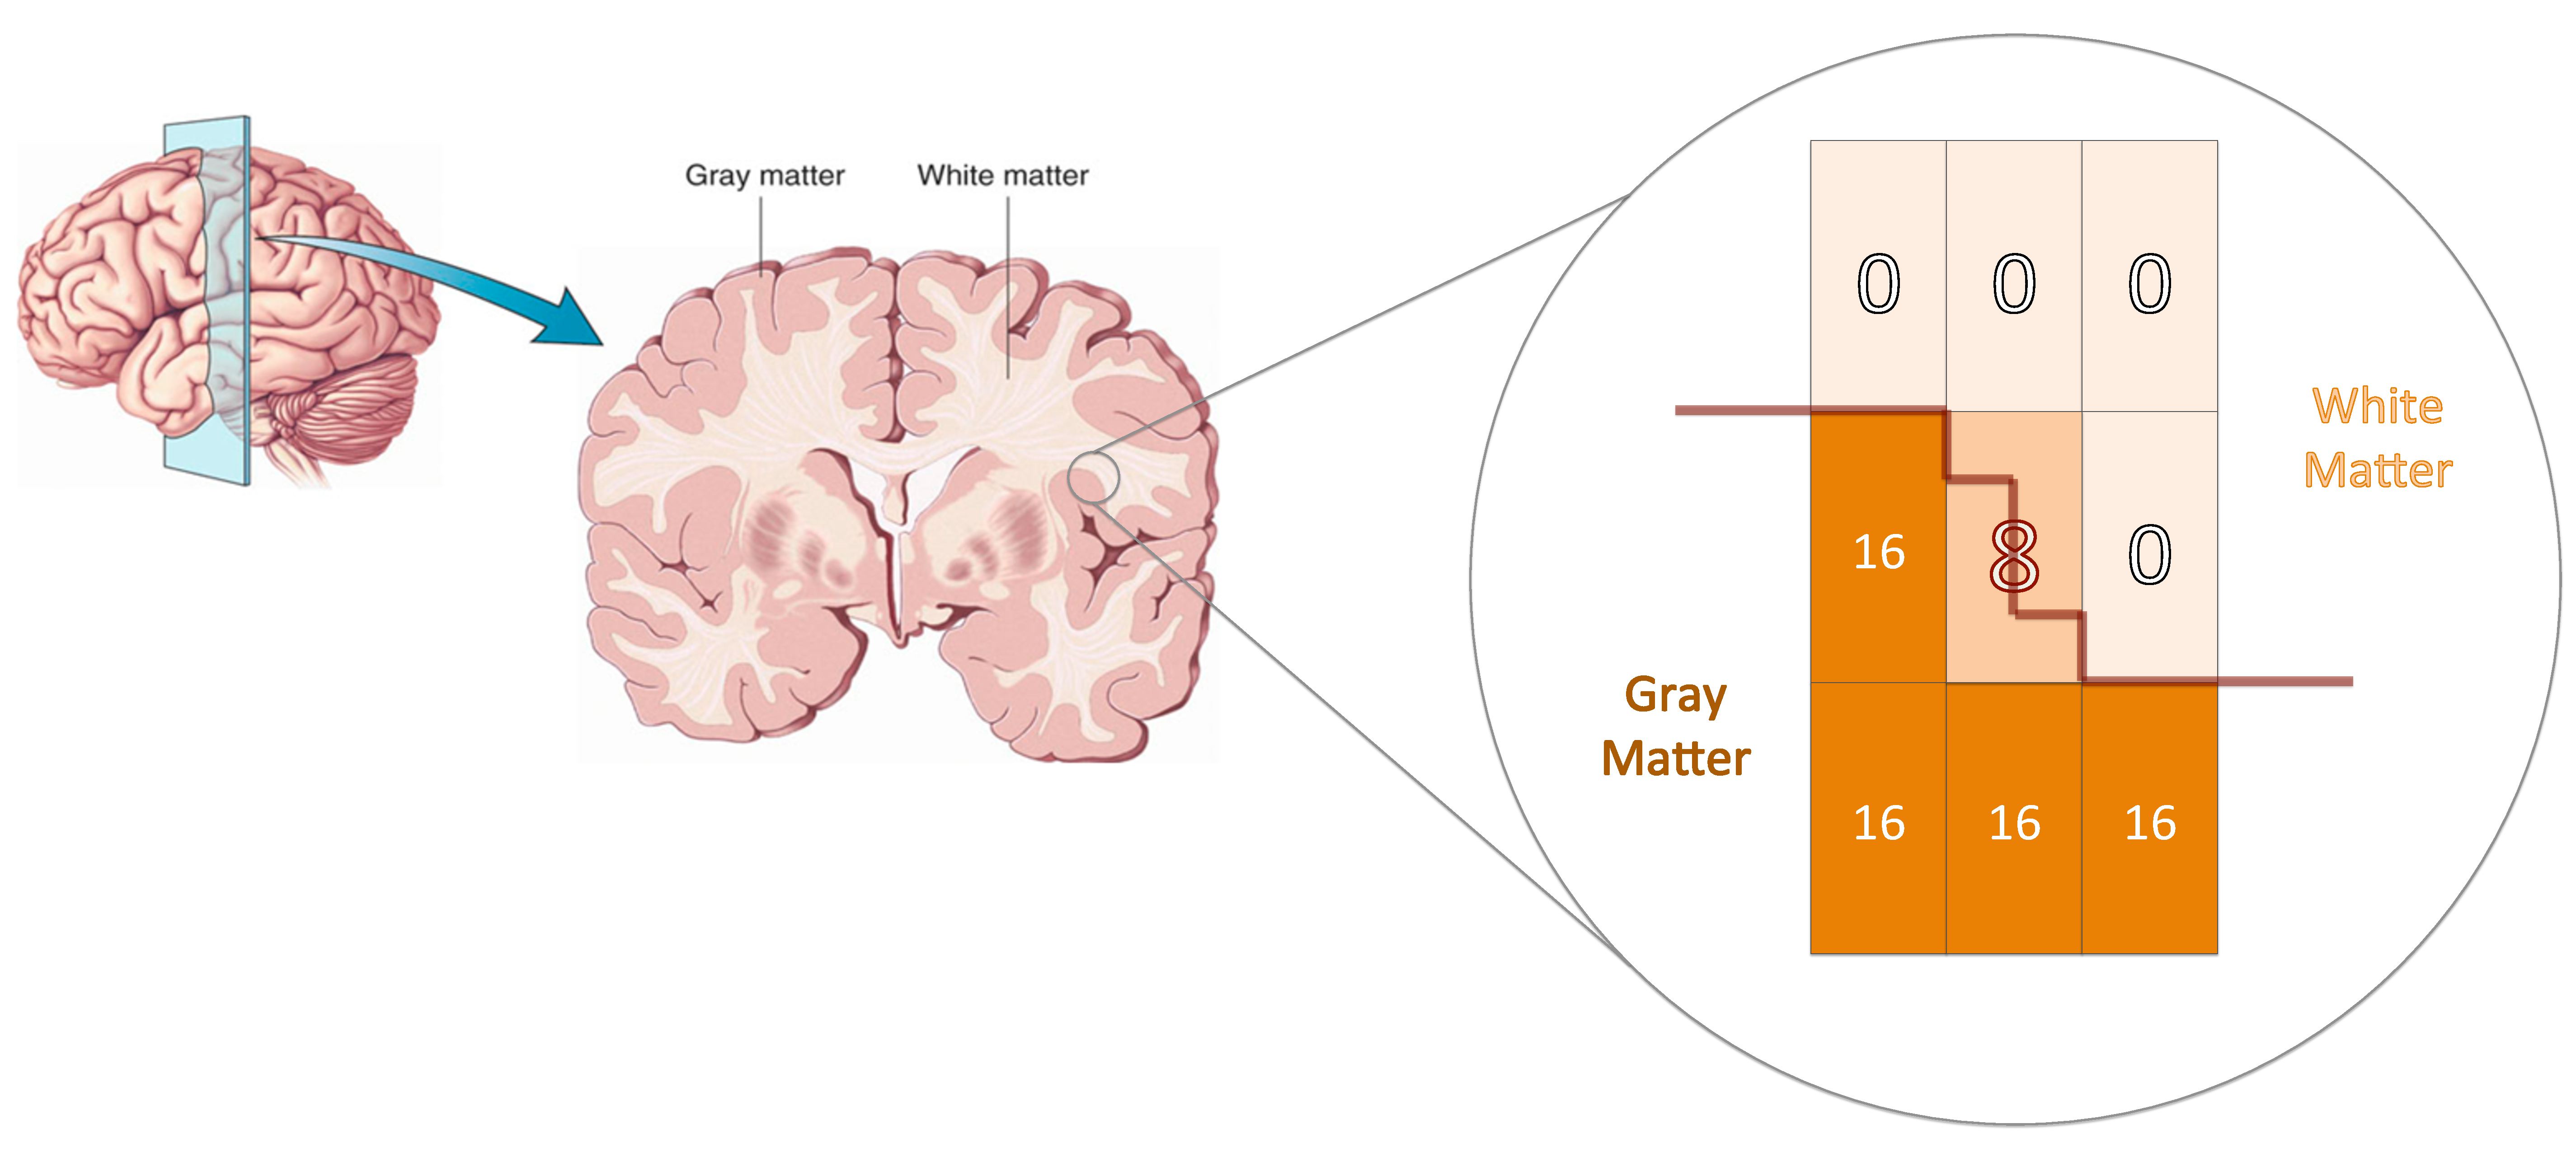
\includegraphics[width=0.8\textwidth]{./Figures/super_resolution1.pdf}
    \end{center}
    \vspace{-15pt}
    \caption{The mismatch between actual anatomical boundaries and voxel borders in an image with low spatial resolution. [brain slice figure from: \textit{http://multiple-sclerosis-research.blogspot.com/}]}
    \vspace{-5pt}
    \label{fig:super_resolution1}
\end{figure}

\noindent As shown in figure \ref{fig:super_resolution2}(a), naively resampling the low resolution data to a higher resolution voxel space only replicates the original values to smaller voxel segments, so it introduces no new information to the output resampled image. Also, the resampled voxels around the tissue boundaries do not have a value consistent with their neighboring voxels.
\newline

\noindent A recent study \cite{Gompf2014} has proposed an algorithm for super-resolved recovery of $2D$ MR images using a mask of edge locations. Their algorithm discretized the mask of edges to the desired resolution as a set of spatial weights $W_{\mu}$ and performs a weighted total variation (TV) recovery:
%--------------------------------
\begin{equation}
  \min _{x}\left| \left| Ax-b \right| \right|^{2}_{2} + \lambda\left| \left| W_{\mu}.\left| \nabla x \right|\right| \right|^{}_{1}
\end{equation}
%--------------------------------
where $x$ is the image to recover, $A$ is the Fourier under-sampling operator, $b$ is the vector of noisy low-pass Fourier measurements, $\lambda$ is a regularization parameter, and $\left| \nabla x \right|$ denotes the magnitude of the discrete gradient of $x$.
\newline

\noindent This study will investigate the use of this idea for super-resolution reconstruction of low resolution diffusion-weight images. Segmentation results in higher spatial resolution provides discretized boundaries that are a very closer estimation to real anatomical boundaries. This study will use these high resolution boundary curves as prior information to recover the super-resolved DWI as shown in figure \ref{fig:super_resolution2}(b).

\begin{figure}[ht!]
    \begin{center}
      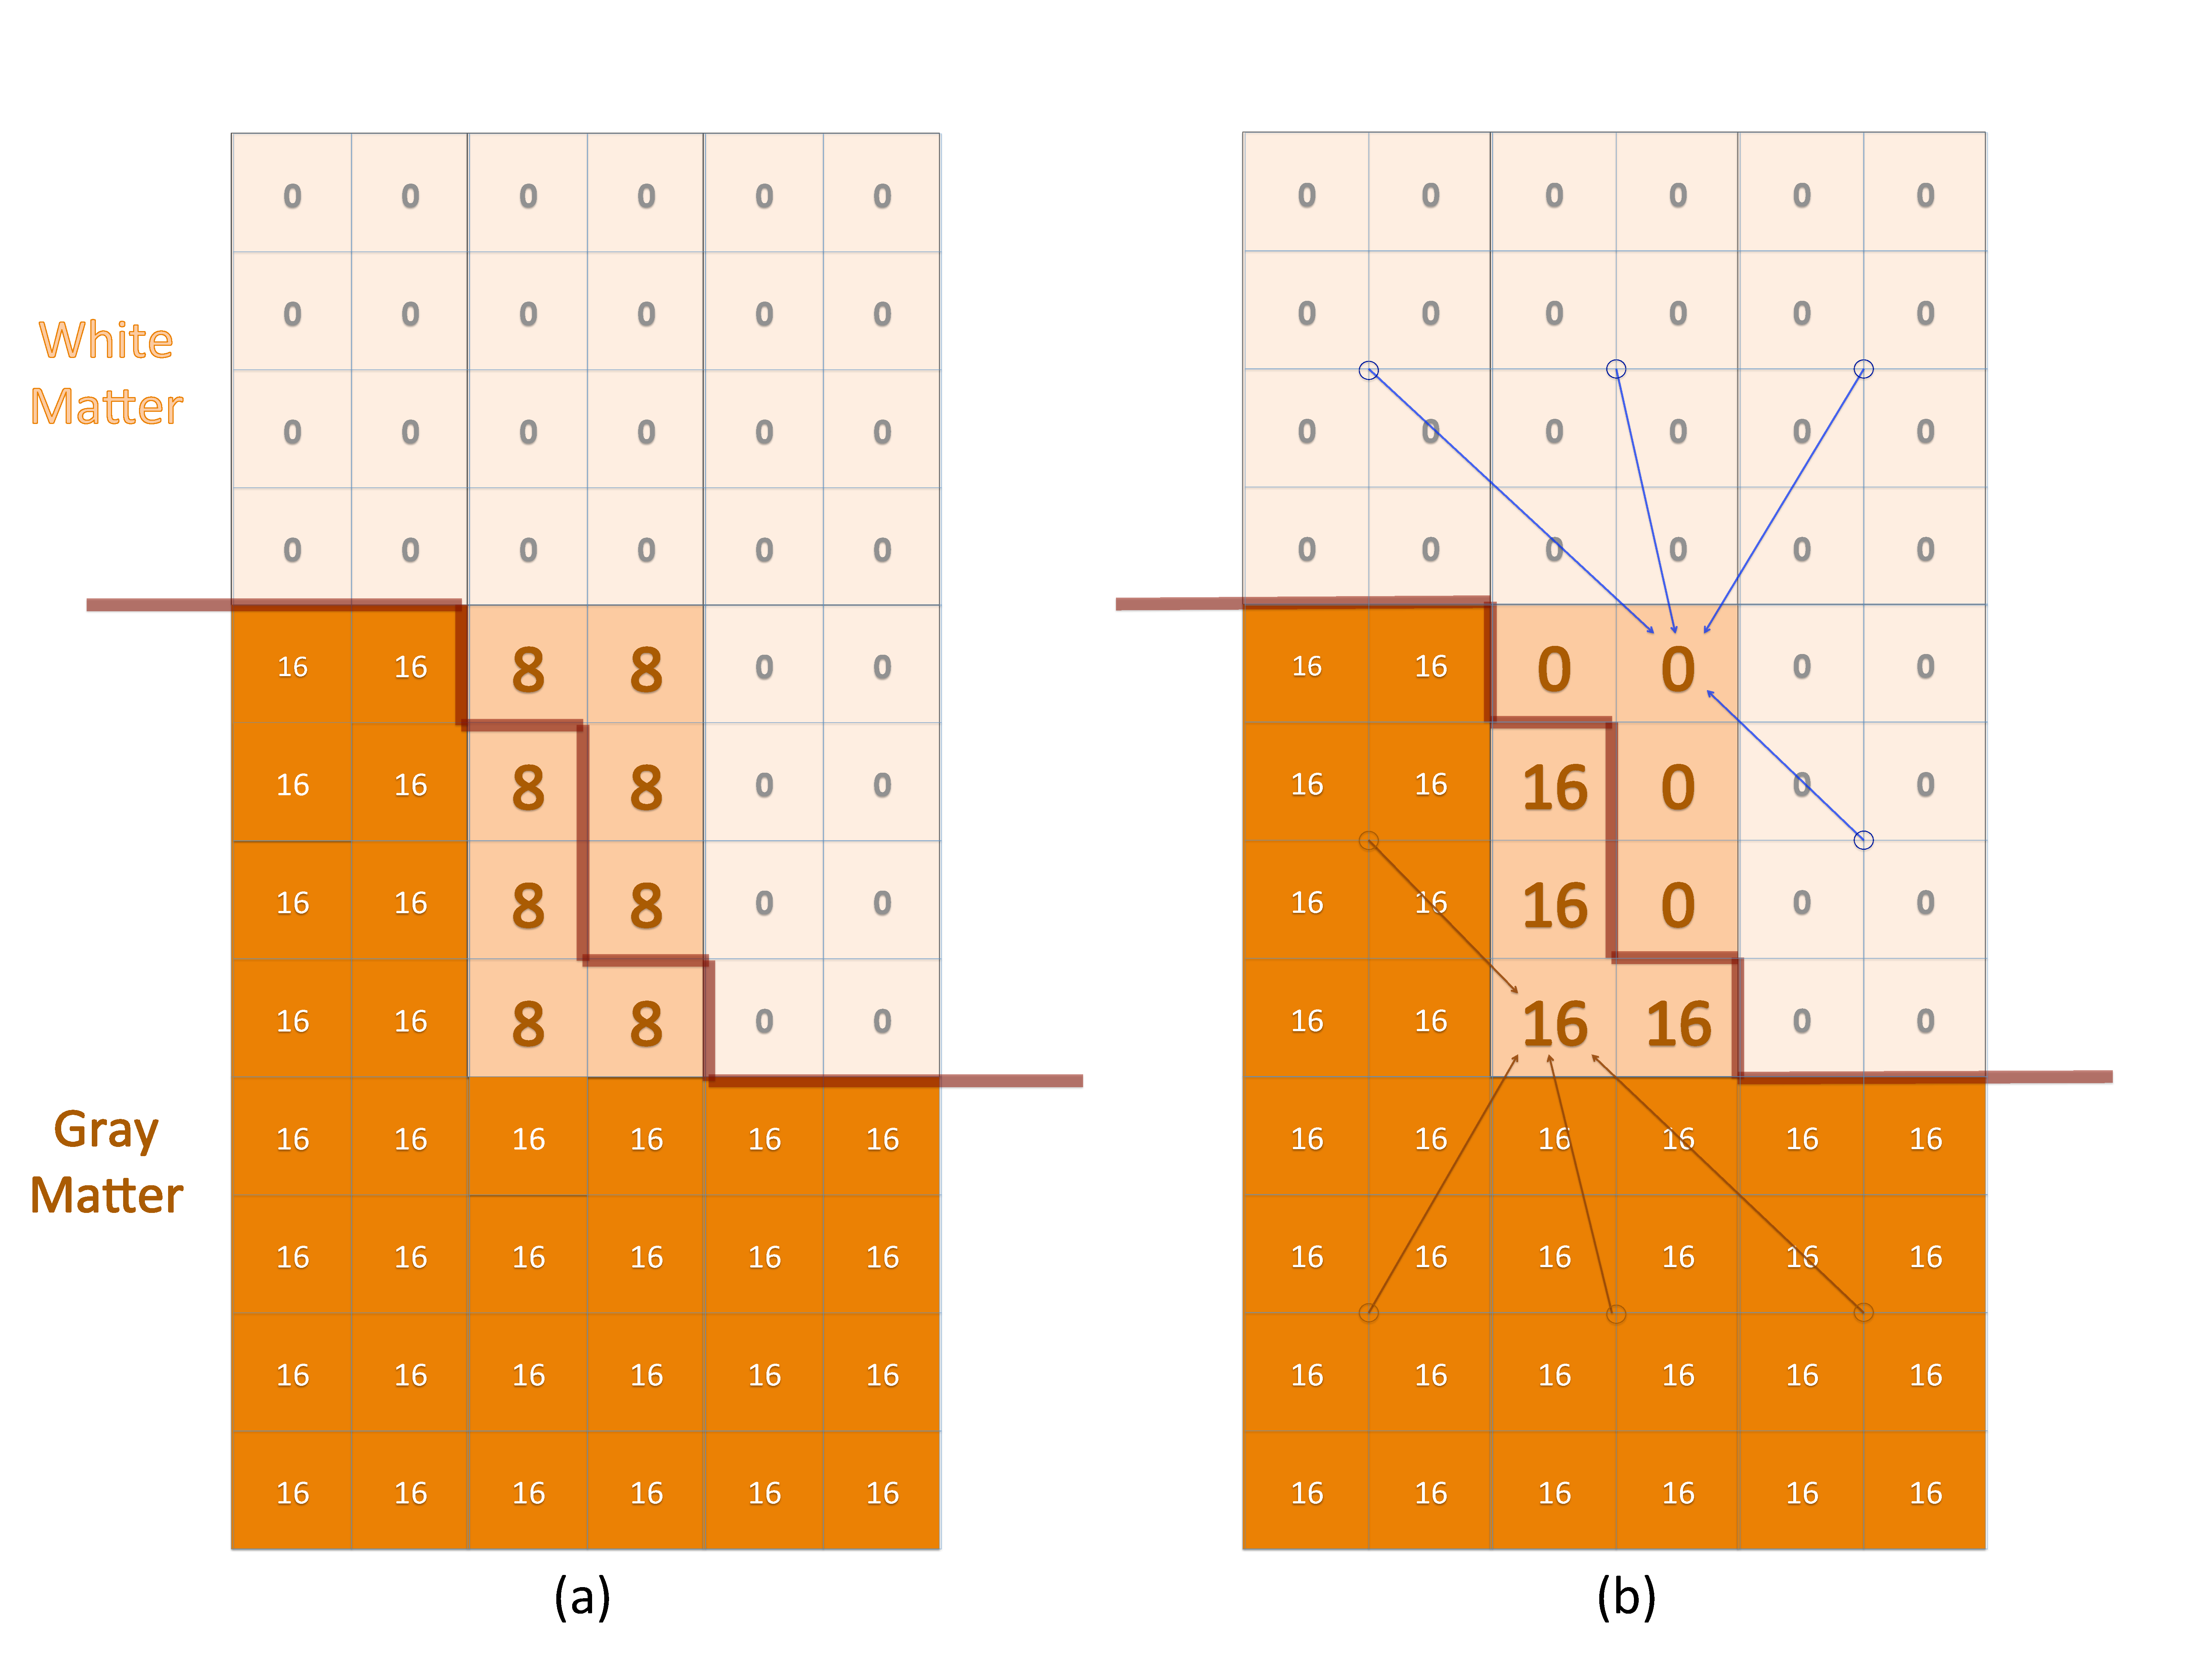
\includegraphics[width=0.8\textwidth]{./Figures/super_resolution2.pdf}
    \end{center}
    \vspace{-15pt}
    \caption{(a) Using basic interpolation techniques to resample the low resolution DWI scan to higher resolution voxel space. It simply replicates the old values to smaller voxel segments. (b) Using high resolution boundary curves as prior information to produce super-resolution reconstruction of DWI scan.}
    \vspace{-5pt}
    \label{fig:super_resolution2}
\end{figure}


\bibliographystyle{unsrt}
\bibliography{biblio}
%\bibliography{biblio_A,biblio_J,biblio_R,misc}

\end{document}


